\section{KI-Module in AMT-Systemen}
\label{sec:ki_integration}
KI-Systeme haben, in den letzten Jahren stark an beliebtheit gewonnen.
AMT-Systeme bilden da keine Ausnahmen.
Vor allem durch die integration von CNNs und RNNs konnten AMT-Systeme zahlreiche Prozesse deutlich verbessern
und neue Errungenschaften in dem Forschungsgebiet erzielen.
Es gibt jedoch auch weitere wichtige KI-Module die in AMT-Systemen häufig genutzt werden
oder zur integration in Planung stehen.
In diesem Kapitel werden genau diese KI-Module stärker behandelt
und deren Aufgaben in der automatischen Musik transkription weiter erläutert.

\subsection{Convolutional Neural Networks}
CNNs sind neuronale Netze, welcher besonders gut räumlich strukturierte Daten analysieren können.
Deshalb werden diese vor allem in der analyse von Bildern genutzt.
Sie können zum Beispiel erkennen, was auf einem Bild genau passiert oder welche Objekte in einem Bild zu erkennen sind.
Auch KIs wie ChatGPT nutzen eine verbesserte Form von CNNs, um Bilder zu analysieren.
Im Fall der Musiktranskription wird als Input Bild ein Spektrogramm verwendet.
Spektrogramme können ähnliche wie zweidimensionale Bilder gehandhabt werden,
da auf diesen auch alle wichtigen Daten des Inputs Audiosignals zu finden sind.
CNNs bestehen aus mehreren verschiedenen Layern.
Einfache CNN Modelle bestehen nur aus 2 bis 5 Layern,
wobei komplexere CNNs aus über tausende Layern bestehen können.
In AMT-Systemen haben die meisten CNNs etwa drei bis zehn Layer.
Diese Layer sind Convolutional Layer (Faltungsschicht), Activation Layer (ReLU), Pooling Layer,
Batch Normalization, Dropout Layer und Upsampling.
Mit jedem Layer kann ein CNN immer abstraktere Merkmale erkennen.
Außer dem Convolutional Layer und Activation Layer sind die anderen Layer jedoch nicht unbedingt notwendig.
Eine Arbeit, welche die stärke, von CNN-Modellen in AMT-Systemen, sehr gut darstellt, heißt \("\)Onsets and frames\("\).
\cite{hawthorne2017onsets}
In dieser Arbeit werden direkt zwei verschieden spezialisierte Teilnetzwerke für Onsets und Sustain der Noten.
Mit diesem System wird die Entwickelung des Forschungsgebietes illustriert.
Insbesondere für polyphone Klaviertranskription ist dieses AMT-System ausgezeichnet.
Im Folgenden werden die verschiedenen Layer eines CNNs, in einem AMT-System, erläutert.

\subsubsection*{Layer eines CNNs}
In dem Convolution Layer werden Filter verwendet.
Filter sind 2D-Matrizen, die aus trainierbaren Gewichten bestehen.
Ein Filter deckt jeweils einen 3x3 Pixel Eingabebereich des Inputbildes ab.
Jeden Filter, den man auf das Bild anwendet,
wird über das gesamte Bild gezogen und analysieren dadurch erstmal jeden Eingabebereich einzeln.
Ein Skalarprodukt aus Filter und Eingabebereich beschreibt dann einen Aktivierungswert.
Aus allen Aktivierungswerten eines Filters entsteht eine Feature Map.
Wenn man Aktivierungswerte miteinander vergleicht,
können somit Patterns und Eigenschaften erkannt werden.
In der Musiktranskription filtert man somit Onsets, Sustains oder harmonische Verläufe heraus.
Zum Beispiel Onsets werden erkannt, wenn es eine plötzliche Energieänderung gibt.
Am Ende bekommt man einen 3D-Tensor raus, welcher alle Feature Maps beinhaltet.

Die Batch Normalization sorgt dafür, das die Aktivierungswerte normalisiert werden.
Jede Feature Map wird dabei einzeln normalisiert.
Dadurch wird Rechenleistung eingespart.
Zudem kann man im Training durch Mini-Batches mehrere Spektrogramme gleichzeitig durch die CNN Struktur leiten.
Dadurch wird das Training schneller und man kommt früher an Ergebnisse.

Es kann passieren das die Summe eines Convolution Layers negativ ist.
Dies kann passieren, wenn stärker gewichtete Filter einen negativen Aktivierungswert herausgeben.
Negative Werte können zu Informationsverlust, von Eigenschaften des Musikstückes, führen.
Um das zu vermeiden werden im Activation Layer, meistens mit der ReLU Funktion,
alle negativen Aktivierungswerte auf 0 gesetzt.
So kann das Netz nichtlineare Beziehungen modellieren.

Als Nächstes wird mit dem Pooling Layer der Rechenaufwand verringert.
Dieser nimmt jede Feature Map einzeln und reduziert deren Matrix zu einer kleineren, standardmäßig eine 2x2, Matrix.
Das erfolgt, indem sich der Pooling Layer zunächst eine
gesamte Feature Map nimmt und diese dann in kleinere Blöcke aufteilt.
Es gibt entweder Max-Pooling oder Average-Pooling.
Je nachdem welche Methode man wählt, wird immer der höchste Wert oder der durchschnittliche Wert extrahiert.
Der extrahierte Wert von jedem Block wird nun in die reduzierte Feature Map zurückgeführt.
Dadurch reduziert man nicht nur Rechenaufwand, sondern vermeidet auch überanpassung.
Wenn das System jeden kleinsten Wert berücksichtigt passt es sich zu sehr an den trainingsdaten an
und kann womöglich andere Daten nicht mehr richtig analysieren.

Der Dropout Layer ist, im gegensatz zu den anderen Layern, nur im Training relevant.
Er schaltet zufällig bestimmte Neuronen aus,
sodass sich Neuronen nicht ausschließlich auf bestimmte andere Neuronen verlassen können.
Somit wird das gesamte neuronale Netzwerk robuster und vielseitiger.

Upsampling ist das Gegenteil von dem Pooling Layer.
Anstatt die Feature Maps zu reduzieren, werden diese wieder hochskaliert.
Dadurch kann man bestimmte Features wieder zeitlich präziser bestimmen,
da die Zeitfenster wieder genauer zum originellen Audiosignal sind.
Meist wird dieser Layer jedoch weggelassen, da er häufig nicht sehr relevant für AMT-Systeme ist.

Ein CNN gibt als letzte Ausgabe einen 3D-Tensor zurück,
welcher aus den Zeitfenster (Frames / T), der Frequenzachsenlänge (F) und der Anzahl der Filter (C) besteht.
\[
\text{CNN-Ausgabe} \in \mathbb{R}^{T \times F \times C}
\]
Meist schließt sich nach einem CNN, in einem AMT-System, ein RNN als Nächstes an.
Dieses kann jedoch nur 1D-Vektoren verarbeiten und nicht einen 3D-Tensor.
Dieser 3D-Tensor wird deshalb vor der Übergabe durch eine Flattening-Operation
zeitschrittweise in 1D-Vektoren umgewandelt.
Dabei wird der Vektor mit einer Dimension von F × C erhalten.
Diese Vektoren werden dann an das folgende RNN weitergeleitet.

\begin{figure}[H]
    \centering
    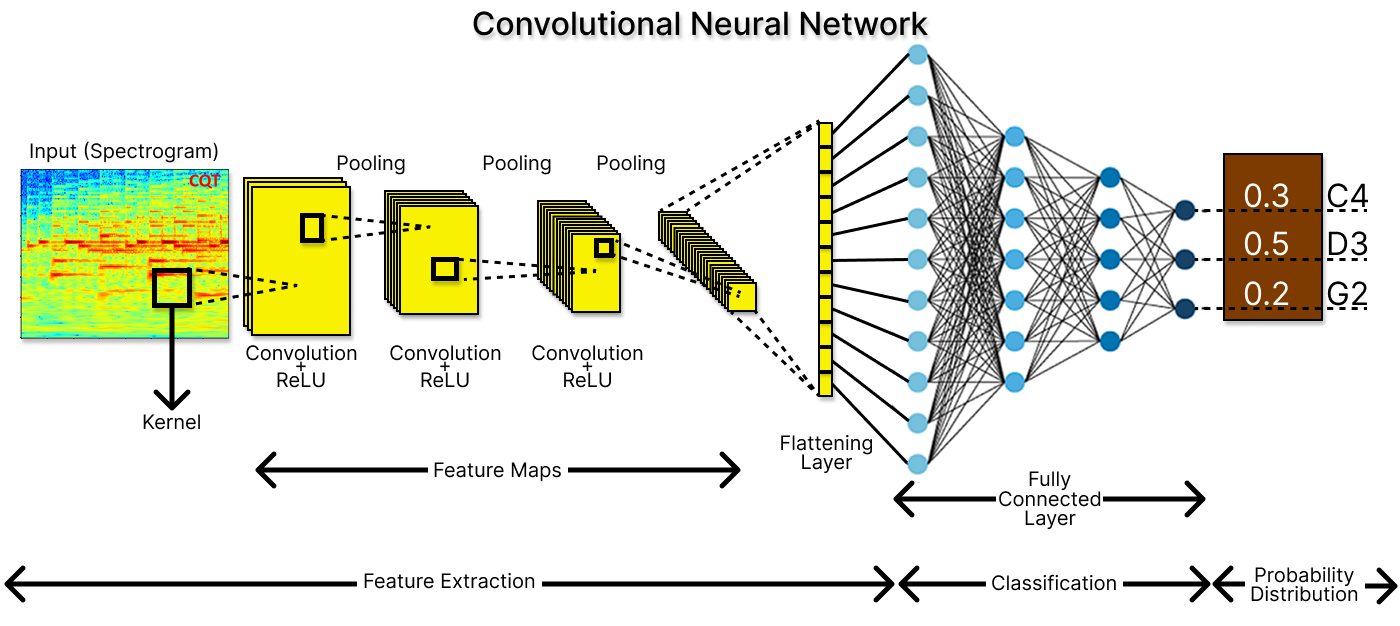
\includegraphics[width=1\textwidth]{Graphics/CNN}
    \caption{Visualisierung eines CNNs zur automatischen Musiktranskription. Eigene Darstellung in Anlehnung an \cite{shahriar2020cnn}}
    \label{fig:cnn-amt}
\end{figure}

\subsubsection*{Geschichtliche Einordnung von CNNs}
CNNs finden Ihren Ursprung im Jahre 1979.
Die erste richtige Architektur für CNNs wurde, unter dem Namen \("\)Neocognitron\("\), veröffentlicht.
\cite{fukushima1980neocognitron}
Dies sollte als Vorreiter für spätere CNN Modelle gelten.
Es dauerte weitere 10 Jahre bis das erste richtige Convolutional Neural Network veröffentlicht wurde.
\cite{lecun1989backpropagation}
Dieses CNN Modell unterscheidet sich speziell in drei bestimmten Punkten zu dem Vorgänger Neocognitron.
In diesem wurde Gradientenlernen durch Backpropagation integriert,
wodurch das gesamte Netzwerk erstmals auf ein gemeinsames Ziel zu trainieren konnte.
Neocognitron besaß zudem, im Gegensatz zu LeCuns CNN,
keine Gewichtsverteilung mithilfe von Filtern, wie es in heutigen CNN Modellen standard ist.
Zudem hatte Fukushima keine praktische Anwendung.
Er hatte die Idee und wie man diese umsetzt, doch durch damalige Verhältnisse war es für ihn schwierig diese umzusetzen.
Für AMT-Systeme wurde CNN jedoch erst ungefähr im Jahre 2015 relevant.
\cite{sigtia2016end}
In dieser Arbeit wurde erstmals polyphone Musikstücke mithilfe von CNNs, und weiteren KI-Modulen, transkribiert.
Seitdem sind CNNs ein wichtiger bestandteil der modernen automatischen Musiktranskription.

\subsection{Recurrent Neural Networks}
RNNs sind neuronale Netze, welche entworfen wurden um Daten mit zeitlicher Struktur zu verarbeiten.
Dabei ist die besonderheit von RNNs das diese ein Gedächtnis haben.
Wenn jetzt in einem AMT-System eine bestimmte Tonabfolge gespielt wurde,
kann sich das RNN diese merken und dementsprechend die fortlaufenden Ausgaben anpassen.
Dies passiert dank den Hidden States.
Dieser stellt das Gedächtnis des RNNs dar und ist einer der wichtigsten Faktoren in einem RNN\@.
Mehr zu den Hidden States werden im Abschnitt-\titleref{itm:hidden} ausführlicher beschrieben.
Dieses Prinzip ist in der Musiktranskription sehr hilfreich,
da jede Note stark von den vorherigen gespielten Noten abhängt.
Takt, Rhythmus, Harmonie und die Melodie eines Musikstückes sind alles gute Beispiele,
warum diese sequenzielle Abfolge so passend in AMT-Systemen ist.

RNNs haben in der automatischen Musiktranskription mehrere Aufgabenfelder.
Je nachdem wie man das RNN trainiert bewältigt dieses alle Aufgaben oder nur einen Teil.
Diese Aufgaben bestehen aus Frame-Glättung (Temporal smoothing), Kontext-Modellierung (Temporal context modeling),
Feature-Zusammenführung (Sequential integration of acoustic features)
und Ausgabevorbereitung (time-distributed output classification).
Diese Aufgaben werden auf jedes Zeitfenster, auf jeden 1D-Vektor des CNNs, angewendet.
Doch bevor man sich auf diese einzelnen Aufgaben konzentrieren kann, muss man noch wissen, was Hidden States sind.

\begin{description}[style=nextline]
\item[Hidden States]\label{itm:hidden}
Hidden States sind das grundlegende Prinzip, warum RNNs funktioniere.
Sie stellen praktisch das Gedächtnis des RNNs dar und helfen somit
anderen Modulen Vorhersagen über bestimmte musikalische Eigenschaften zu treffen.
Für jeden 1D-Vektor, den das CNN liefert, wird ein Hidden State erstellt.
Diese werden sequenziell nacheinander, mit abhängigkeit des vorherigen Hidden States, definiert.
\[
\mathbf{h}_t = f(\mathbf{x}_t, \mathbf{h}_{t-1})
\]
In Hidden States ist das Wissen der vorherigen Zeitfenster über zeitliche Muster, wie Sustain und Akkordstruktur.
Sie alleine können jedoch noch keine eigene Entscheidung über bestimmte Noten fallen.
Dafür müssen andere Module die Informationen der Hidden States später richtig verwerten.
Jeder Hidden State hat eine Anzahl von Dimensionen, welche gleich der Anzahle der Neuronen in einem RNN ist.
\end{description}

\subsubsection{Grundstruktur eines RNNs}
Bei der Frame-Glättung bekommt das RNN als Input die Aktivierungswerte des Zeitfensters.
Es betrachtet diese mit Kontext zu den vorherigen Zeitfenstern, um falsche vorhersagen auszuschließen.
Das CNN hat dem RNN schon Vorhersagen für bestimmte Noten gegeben.
Diese könnten jedoch fehlerhaft.
Zum Beispiel kann die Note C4 für den Frame 6 und 8 aktiv sein,
aber bei dem Frame 7 hat das CNN diese Note nicht als aktiv angesehen.
Es ist sehr unwahrscheinlich, das eine Note für nur einen Frame ausfällt.
Solche Arten von Fehlern verarbeitet das RNN und glättet dementsprechend die vorher vom CNN gelieferten Daten.
Dadurch ist der Ton C4 auch im Frame 7 aktiv.

Die Kontext-Modellierung ist etwas komplizierter als die Frame-Glättung.
Als Input bekommt diese auch die 1D-Vektoren des CNNs.
In der Kontext-Modellierung werden größere zeitliche Zusammenhänge betrachtet.
So kann die Kontext-Modellierung, mithilfe des Hidden States,
den Notenverlauf oder auch die länge einer Note vorhersehen.
Je nach den Trainingsdaten ist es zum Beispiel üblicher das auf C4 ein D3 folgt,
was durch die Kontext-Modellierung angepasst wird.
Dies ist aber immer stark von der Musikrichtung und Musikern abhängig, welche in den Trainingsdaten vorhanden sind.
Jazz und Pop oder Bach und Taylor Swift unterscheidet sich der style der Tonabfolge extremst.
Zudem wird Onset, Sustain und Offset stabilisiert.
Durch vorherige Beispiele weis die Kontext-Modellierung,
wie lange eine bestimmte Note andauern wird und kann so das Offset der Note einschätzen.
Als Output bekommt man Kontextabhängige Vektoren.
Sie haben die gleiche Struktur wie die 1D-Vektoren vom CNN, sind aber entsprechend dem Kontext angepasst.

Die Feature-Zusammenführung ist der letzte wichtige interne Schritt eines RNNs.
Bei diesem werden aus, lokalen alleinstehenden, Informationen eines Zeitfensters, konkrete musikalische Ereignisse.
Dadurch schreibt das RNN Ereignisse, wie Akkorde, Noten, Onsets und vieles mehr, heraus.
Dafür muss die Feature-Zusammenführung sich die einzelnen 1D-Vektoren als eine folge von Events anschauen.
Dies passiert wiedermal über den Hidden State.
Das wird vor allem wichtig, wenn man später eine MIDI-Datei ausgeben möchte,
da in dieser auch die einzelnen musikalischen Ereignisse aufgeschrieben sind.
Als Output bekommt man kontextreiche Vektoren.
Diese Vektoren sind, durch die vorherigen Module angepasste und verbesserte, Hidden States.

Die Ausgabevorbereitung ist der letzte Schritt des RNNs,
wodurch nun die gesammelten Daten zu echten musikalischen Ereignissen zusammengefügt werden.
Als Input werden die, durch die Feature-Zusammenführung verbesserten, Hidden States genutzt.
Zunächst werden diese durch ein Fully Connected Layer geschickt.
\[
\mathbf{z}_t = W \cdot \mathbf{h}_t + \mathbf{b}
\]
Ein Fully Connected Layer ist ein Klassifikator, welcher den Hidden States auf eine gewünschte Dimension bringt.
Wenn man zum Beispiel Klaviertasten vorhersagen möchte werden alle Hidden States auf mit 88 Dimensionen ausgestattet.
Bei MIDI-Dateien wären es 128 Dimensionen.
Die Werte, welche aus dem Fully Connected Layer stammen, sind jetzt noch nicht richtig interpretierbar.
Um diese als konkrete und normalisierte Wahrscheinlichkeiten darstellen zu können,
wird eine Aktivierungsfunktion eingesetzt.
Mit, zum Beispiel, der Sigmoid-Funktion als Aktivierungsfunktion,
können alle Werte normiert in einem Bereich zwischen 0 und 1 gebracht werden.
Sagen wir, wir wollen jetzt die gespielten Klaviertasten vorhersagen.
Dann hat jeder Hidden State jetzt für alle Klaviertasten einen eigenen Wert mit einer Wahrscheinlichkeit,
das diese Taste zu dem gewählten Moment gespielt wurde.
Zu guter Letzt muss jetzt ein Threshold bestimmt werden.
In polyphonen Musikstücken können immer mehrere Noten gleichzeitig erklingen,
weshalb man nicht einfach die Note mit der höchsten Wahrscheinlichkeit auswählen kann.
Deshalb nutzt man einen Threshold, zum Beispiel bei 50\%,
welcher bestimmt wie viel Prozent eine Note braucht um als aktiv zu gelten.
Durch Postprocessing können einige Eigenschaften wie Rauschen noch herausgefiltert werden.
Postprocessing ist jedoch nicht relevant für den KI-Ablauf.
Wenn man zufrieden mit dem Ergebnis ist, kann man dieses jetzt in das gewünschte Output-Format,
standardmäßig MIDI-Dateien, einfügen.

Heutzutage sind RNNs sind nur die grundlegende Struktur.
Basierend auf dieser Struktur gibt es einige bessere Systeme,
welche Aktiv in AMT-Systemen und anderen KI-Systemen genutzt werden.
Zwei dieser Systeme sind Long Short-Term Memory's (LSTM) und Bidirektionale RNNs (BiRNN).
Diese werden im jetzt folgendem Abschnitt ausführlicher erklärt.

\subsubsection{Long Short-Term Memory}
LSTMs sind verbesserte RNNs.
Diese kontrollieren durch Gates besser, welche Daten sie wirklich in den Hidden State speicher möchten.
Dadurch kann man das neuronale Netz noch weiter an seine gewünschten Ansprüche anpassen.
Ein normals RNN berechnet einen Hidden State mit folgender Formel:
\begin{equation*}
h_t = \tanh(W x_t + U h_{t-1} + b)
\end{equation*}
Dabei werden alle Daten, egal ob sinnvoll oder nicht, miteinander kombiniert.
Somit kann sich das RNN langfristig schwieriger Information merken.
Wenn zum Beispiel im 2\. Hidden State ein Onset erkannt wurde, kann der 20\. Hidden State
sich das schlechter merken, da ganz viele andere Informationen mitgeschrieben wurden.
LSTMs lösen dieses Problem mit Forget, Input und Output Gates und dem Cell State.
Der Cell State stellt das Langzeitgedächtnis des LSTMs dar.
Er berechnet sich aus den 3 Gates.
Das Forget Gate bestimmt, welche Informationen aus dem vorherigen Cell State gelöscht werden sollen.
Das Input Gate bestimmt, welche neuen Inhalte aus dem neuen Zeitfenster aufgenommen werden.
Dabei ist der Cell-candidate die Datenmenge, welche zum Speichern, durch das Input Gate, vorgeschlagen wird.
Das Output Gate bestimmt, welcher Teil des Cell States zu dem neuen Hidden State hinzugefügt wird.
\begin{align*}
f_t &= \sigma(W_f x_t + U_f h_{t-1} + b_f) \quad &&\text{(Forget Gate)} \\
i_t &= \sigma(W_i x_t + U_i h_{t-1} + b_i) \quad &&\text{(Input Gate)} \\
o_t &= \sigma(W_o x_t + U_o h_{t-1} + b_o) \quad &&\text{(Output Gate)} \\
\tilde{c}_t &= \tanh(W_c x_t + U_c h_{t-1} + b_c) \quad &&\text{(Cell-candidate)} \\
c_t &= f_t \odot c_{t-1} + i_t \odot \tilde{c}_t \quad &&\text{(Cellstate)} \\
h_t &= o_t \odot \tanh(c_t) \quad &&\text{(Aktueller Hidden State)}
\end{align*}
Dadurch kann sich ein LSTM die verschiedenen musikalischen Ereignisse,
über das gesamte Audiosignal, besser im Zusammenhang merken.

\subsubsection{Gated Recurrent Units}
GRUs sind, neben LSTMs, eine weitere spezielle Art von RNNs.
\cite{chung2014empirical}
Sie wurden erfunden, um bestimmte Probleme von RNNs zu lösen.
Insbesondere das Problem des \("\)Vanishing Gradients\("\) sollten GRUs lösen.
GRUs steuern mithilfe von Gates, welche Informationen gemerkt und welche vergessen werden sollen.
Sie sind, im gegensatz zu LSTMs, eher für kleinere Aufgaben geeignet.
Dafür sind sie weniger fehleranfällig und haben ein schnelleres Training.

Ein GRU besitzt zwei Gates.
Sie haben, genau wie bei LSTMs, die Aufgabe das Gedächtnis des KI-Models zu verwalten.
Das Reset Gate schaut sich den alten Hidden State an und entscheidet,
wie viel von diesem Wissen in den neuen Hidden State mit einfließt.
Das Update Gate hingegen sieht den aktuellen Hidden State und überlegt,
welche Informationen davon in das Langzeitgedächtnis mit einbezogen werden.
Danach führt das Update Gate die beiden überarbeiteten Hidden States zusammen zum neuen Hidden State.

Das Problem des Vanishing Gradients bezieht sich auf das Gedächtnis des KI-Models.
Das Problem tritt in den Trainingsphasen von neuronalen Netzen auf.
Die Gradienten werden bei der Backpropagation immer kleiner,
wodurch die betroffenen Schichten im Netzwerk fast gar nichts lernen.
Die Gradienten werden kleiner, da eine Aktivierungsfunktion immer einen Wert zwischen 0 und 1 zurückgibt.
Ein Gradient wird mit der Ableitung der Aktivierungsfunktion multipliziert, wodurch er gleichzeitig kleiner wird.
Desto tiefer das Netzwerk ist, desto mehr Schichten müssen die Gradienten durchlaufen.
Mit jeder Schicht wird der Gradient somit exponentiell kleiner.
Die führt dazu, dass das betroffene KI-Modell sich keine Informationen Langzeitig merken kann.
Bei GRUs wird das Problem des Vanishing Gradients durch die Gates gelöst.
Sie stellen eine gewichtete Mischung aus altem und neuen Hidden State dar.
Dadurch wird der Gradient nicht ständig verkleinert
und wichtige Informationen können über einen langen Zeitraum gespeichert werden.

\subsubsection{Bidirektionale RNNs}
Um ein noch besseres Ergebnis zu erhalten, kann man auch ein Bidirektionales RNN nutzen.
Dieses besteht aus zwei RNNs.
Eines liest die Zeitfenster von vorne und das andere von hinten ab.
Dadurch bekommt man die doppelte Menge Hidden States und die gesamte Vorhersage wird sehr viel robuster.
\[
\mathbf{h}_t = \left[ \overrightarrow{\mathbf{h}}_t \ ;\ \overleftarrow{\mathbf{h}}_t \right]
\]
Auch in AMT-Systemen sind Bidirektionale RNNs sehr hilfreich,
da musikalische Ereignisse auch eine klar verständliche Abhängigkeit, von der Zukunft in die Vergangenheit aus, haben.
Das gleiche Prinzip kann man auch auf LSTMs oder GRUs einsetzen.
Bidirektionale RNNs sind noch robuster, aber dafür ist der Rechenaufwand bei weitem höher.
Ein Bidirektionales RNN kann man auch in folgender Arbeit finden.
\cite{hawthorne2017onsets}

\subsubsection*{Geschichtliche Einordnung von RNNs}
Die Geschichte von Recurrent neural networks reicht bis in das Jahr 1990 zurück.
\cite{elman1990finding}
In dieser Arbeit wurde erstmals die Idee der Rückkopplung eingebaut,
wodurch der Output eines Neurons als zusätzliche Eingabe im nächsten Zeitfenster genutzt wird.
Das resultierte später in den Hidden States.
Diese Arbeit baute den Grundstein für alle weiterführenden RNNs.
Eine weitere wichtige Arbeit über RNNs ist die folgende.
\cite{jordan1997serial}
Diese Arbeit über RNNs wurde, offiziell im Jahre 1997, publiziert,
obwohl sie schon 1986 als ein technischer Bericht veröffentlicht war.
Zudem wurde, im Jahre 1997, das erste Bidirektionale RNN
\cite{schuster1997bidirectional}
und das erste LSTM erfunden.
\cite{hochreiter1997long}
Erst über ein Jahrzehnt später wurde das erste GRU entwickelt.
\cite{chung2014empirical}
RNNs fanden ihren Weg in die automatische Musiktranskription, fast zeitgleich zu CNNs, im Jahre 2015.
\cite{sigtia2015hybrid}
Für LSTMs dauerte die Einbindung in AMT-Systeme etwas länger.
Erst im Jahre 2016 wurde ein LSTM in einem AMT-System eingefügt.
\cite{sigtia2016end}
Dahingegen wurde das erste Bidirektionale RNN erst Ende 2017 in ein AMT-System integriert.
\cite{hawthorne2017onsets}
Noch ein Jahr später wurde das erste Mal auch ein GRU in einem AMT-System genutzt.
\cite{jung2018adaptive}

\subsection{Transformers}
Transformer sind eine, von Google entwickelte Deep-Learning Architektur,
die mit dem Prinzip der Self-Attention, zur natürliche Sprachverarbeitung (NLP) genutzt wird.
Auch Transformer verarbeiten die Daten, wie ein LSTM, sequentiell.
Jedoch wurde zu dieser Verarbeitung noch der Attentionmechanismus hinzugefügt,
welcher der grundlegende Baustein eines Transformer-Modells ist.
Die Architektur eines Transformers besteht grundlegend aus 3 Bausteinen.
Diese 3 sind Input Embedding + Position Encoding, der Self-Attention Layer und der Feedforward Layer.
Input Embedding und Position Encoding nur einmalig am anfang des Transformers durchgeführt.
Dahingegen werden Self-Attention und Feedforward mehrmals hintereinander aufgerufen.
Dies passiert grundsätzlich 6-, 12- oder 24-mal, wodurch das Transformer-Modell an Layer gewinnt.
Dieser Schritt wird so oft wiederholt, damit der Transformer immer komplexere musikalische Strukturen erkennen kann.
Als Nächstes werden die einzelnen Schritte eines Transformers näher erläutert.

\subsubsection{Input Embedding und Position Encoding}
Zunächst müssen die Daten, welche der Transformer verarbeiten soll in das richtige Format für diesen umgewandelt werden.
Dafür ist das Input Embedding zuständig.
Tokens sind einzelne Datenpunkte wie zum Beispiel kleine Wörter wie \("\)hallo\("\).
Wenn man zum Beispiel bei ChatGPT die Anfrage stellt \("\)Wie alt sind die Planeten unseres Sonnensystems\("\),
dann wird zwar das Wort \("\)alt\("\) als ein Token gespeichert, aber längere Wörter wie \("\)Sonnensystem\("\)
werden aufgeteilt in \("\)Sonn\("\) und \("\)ensystem\("\).
Je nach Tokenizer-Version, die der jeweilige Transformer nutzt, kann dies jedoch abweichen.
Unser Beispielsatz nutzt, alleine für die Wörter, 9 Tokens.
Tokens können auch einzelne Satzzeichen oder Symbole sein.
Für verschiedene Transformer Modelle gibt es immer eine maximale Tokenanzahl,
bei GPT-3.5 sind es um Beispiel ungefähr 4000 Tokens.
Diese Tokens sind für den Input und Output.
Heißt, wenn der Input zu viele Tokens nutzt, gibt es weniger Tokens für den Output.
Dies ist jedoch häufig, wie man an der Menge der Tokens für unseren Beispielsatz sehen kann, kein größeres Problem.
In AMT-Systemen stellen Tokens Zeitfenster (Frames) oder Musik-Events (Onsets etc.) dar.
Jedoch können diese von einem Transformer nicht verarbeitet werden,
weshalb sie durch Input Embedding erstmals in Vektoren  umgewandelt werden.
Dies passiert über eine Embedding-Matrix, welche die einzelnen Tokens in den Vektorraum einbettet.
\[
Embedding-Matrix \in \mathbb{R}^{Maximale Tokenanzahl \times Embedding-Dimension}
\]
Tokens, welche ähnliche musikalische Eigenschaften speichern, werden im Vektorraum näher beieinander gespeichert.
Das Modell kann die Tokens richtig einordnen durch die gesammelten Daten im Training.

Nun sieht der Transformer die Tokens trotzdem nur als zahlreiche Vektoren, ohne Rheinfolge, an.
Um den Tokens einen Sinn zu geben, müssen diese eine explizite Position erhalten.
Das wird durch Position Encoding gemacht.
Durch zwei Funktionen, eine Sinus und eine Cosinus, wird für jeden Token ein Positionsvektor berechnet.
Dadurch kann der Transformer die relative Position, verschiedener Tokens,
gut miteinander vergleichen und zugleich wiederkehrende Muster erkennen.
Danach wird der Positionsvektor dem Tokenvektor aufaddiert.
Moderne Transformer besitzen manchmal auch gelernte Position Embeddings,
wodurch die Positionen schon durch das Training bekannt sind.
Diese Vektoren werden, als Input, weiter an den Transformer geleitet.

\subsubsection{Self-Attention Layer}
Jeder Input-Vektor wird einzeln behandelt.
Durch Self-Attention kann sich jetzt jeder Vektor merken, welche anderen Vektoren für sich selber relevant sind.
Zunächst wird jeder Input-Vektor in 3 verschiedene Vektoren umgewandelt.
Diese Vektoren heißen Query, Key und Value.
\begin{itemize}
  \item \textbf{Query ($Q$)}: Bestimmt, auf welche Informationen aus anderen Tokens das Modell aktuell achten möchte.
  \item \textbf{Key ($K$)}: Zeigt anderen Tokens, was dieser Input-Vektor anderen Tokens, für Informationen, anbieten kann.
  \item \textbf{Value ($V$)}: Enthält die tatsächlichen Informationen des Input-Vektors.
\end{itemize}
Als Nächstes wird der Attention Score berechnet.
Durch diesen wird die Kompatibilität zu anderen Tokens berechnet.
Als Ergebnis bekommt man, für jeden Token, eine Matrix.
Jeder Wert in dieser Matrix steht für die Ähnlichkeit zwischen zwei verschiedenen Tokens.
Diese Werte sind die Attention Weights.
Durch Softmax werden diese Werte normalisiert.
Als Letztes werden diese Attention Weights mit den Value-Vektoren verbunden.
\[
\text{Output} = \text{Attention Weights} \times \text{Value Vektoren}
\]
Nun können die einzelnen Tokens sich besser auf die Tokens fokussieren, welche wirklich wichtig für deren Ergebnis sind.

\subsubsection{Feedforward Layer}
Der Feedforward Layer stammt von der Idee eines Feedforward neuronalen Netzwerks (FNN).
Dieses neuronale Netz verläuft immer nur in eine Richtung und hat keine Rückkopplung.
Das heißt jeder Token wird für sich alleine, nacheinander, umgeschrieben.
Das funktioniert so, da die jeweilige Gewichtung schon im Self-Attention Layer stattgefunden hat.
Im Feedforward Layer passiert dann folgendes.
Zunächst werden die Vektoren, welche aus dem Self-Attention Layer stammen,
mit einer Gewichtsmatrix auf eine höhere Dimension transformiert.
Durch die erhöhung der Dimension bekommt das Netzwerk mehr Freiraum Informationen voneinander zu trennen
und komplexere Zusammenhänge zu modellieren.
Durch eine Aktivierungsfunktion, zum Beispiel ReLU, erlernt das Modell jetzt nichtlineare Abhängigkeiten.
Diese Aktivierungsfunktion gehört zu dem Hidden Layer des FNN.
Ein FNN kann mehrere Hidden Layer besitzen, welche alle die Input-Werte in irgendeiner Form verändern.
Als Nächstes wird der Vektor wieder auf seine ursprüngliche Dimension zurückprojiziert,
wodurch nur die wichtigsten Informationen erhalten bleiben.
Mathematisch sieht der Feedforward Layer folgendermaßen aus:
\[
y_t = \text{FFN}(x_t) = \left( x_t W_1 + b_1 \right) \xrightarrow{\text{ReLU}} W_2 + b_2
\]
\begin{itemize}
  \item $x_t$: Eingabevektor des Tokens.
  \item $W_1, W_2$: Gewichtsmatrizen, zuständig für Dimensionserweiterung und -reduktion.
  \item $b_1, b_2$: Bias-Vektoren der jeweiligen linearen Projektionen.
  \item $\left( x_t W_1 + b_1 \right)$: Ergebnis der ersten linearen Projektion.
  \item $\text{ReLU}$: Aktivierungsfunktion zur Einführung von Nichtlinearität.
  \item $y_t$: Ausgabewert des Feedforward Layers für das Token.
\end{itemize}

\subsubsection*{Geschichtliche Einordnung von Transformern}
Das erste Transformer-Modell wurde im Jahre 2017 erfunden.
\cite{vaswani2017attention}
Durch den Self-Attention Layer wurde die sequenzielle Modellierung von Daten revolutioniert.
Leider dauerte es noch lange bis der erste Transformer auch in AMT-Systemen genutzt wurde.
Das liegt an mehreren Gründen.
Einerseits gibt es im gegensatz zu Natural Language Processing (NLP) viel weniger Datensätze zum Lernen.
Transformer trainieren auf einem globalen Level und brauchen daher eine große Menge an Datensätzen.
Die Rechenkosten von Transformer sind auch weitaus höher als andere Systeme wie CNN und RNN.
Zudem lag der Fokus bei AMT-Systemen für eine sehr lange Zeit überwiegend bei CNN und RNN basierenden Systemen,
da diese Anwendungsfälle bekannter waren in AMT-Systemen.
Das größte Problem war jedoch wahrscheinlich die Anpassung.
Transformer Modelle waren einfach nicht dafür ausgelegt Musikspezifische Daten zu verarbeiten.
In der Musiktranskription wird immer mit langen Sequenzen, ein gesamtes Musikstück, gearbeitet.
Spezielle Transformer Modelle für diesen Anwednugnsfall mussten noch programmiert werden.
Die ersten Ansätze für Transformer in AMT-Systemen wurden zwischen den Jahren 2021 und 2023 erstellt.
Eine der ausschlaggebendsten Modelle war der Music Transcription Transformer (MT3),
welches von Magenta/Google Brain erstmals im Jahre 2022 veröffentlicht wurde.
\cite{gardner2021mt3}
Dieses spielt eine große Rolle in der Transformer-basierten automatischen Musiktranskription,
da es das erste weit verbreitete Multi-Task-Transkriptionsmodell ist.
Eine der Letzten bedeutenden Errungenschaften zu Transformern und Musiktranskription ist das
YourMT3+ Modell, indem die MT3-Architektur noch weiter verbessert wurde.
\cite{chang2024yourmt3}

\subsection{Potentielle KI-Module}
CNNs und RNNs oder Transformer Modelle wie MT3 werden überwiegend in AMT-Systemen eingebunden,
wenn es sich um KI integration handelt.
Jedoch gibt es noch andere KI-Modelle, die auch ab und zu in AMT-Systemen integriert werden.
Diese gehen, bei der Musiktranskription, ganz anders vor als die vorgestellten Module.
Je nach KI übernehmen sie auch eine ganz andere Aufgabe.
Im folgenden Abschnitt werden einige von diesen, eher experimentellen, KIs vorgestellt.
Wir fangen dabei bei der am meisten erprobten KI an,
sodass die letzte KIs nur theoretisch, für die Musiktranskription, besprochen worden.

\subsubsection*{Variational Autoencoder}
Variational Autoencoder (VAE) ist ein KI-Modell, welches komplexe Daten in eine verdichtete Form überführt
und durch Wahrscheinlichkeiten bestimmte Muster vorhersagen kann.
\cite{kingma2019introduction}
Dabei ist wichtig das VAE kein alleinstehendes KI-Modell ist,
sondern eher als zusatz gilt um bestimmte Bereiche zu verbessern.
In der Musiktranskription könnte ein VAE zum Beispiel bei der Mehrdeutigkeit von Musik helfen.
Wenn mehrere Instrumente spielen ist es schwer die genauen Noten herauszuschreiben.
Da VAEs, anders als CNNs oder RNNs, als ausgabe keine eindeutigen Noten herausgeben,
sondern eine Wahrscheinlichkeit, könnte dies helfen die entscheidung, welche Note gerade spielt, robuster zu gestalten.
Dadurch das sich VAEs nur eine wahrscheinliche Version der Musik, aus den Daten,
extrahieren könnte man auch kreative Variationen des Musikstückes damit bilden.
Die Methode, welche in VAEs genutzt wird, fand Ihren Ursprung in folgendem Paper.
\cite{kingma2013auto}

\subsubsection*{Graph Neural Network}
Graph Neural Network (GNN) ist ein KI-Modell, welches dazu dient Daten, mit abhängigkeit voneinander, zu verarbeiten.
Diese Daten werden in einem Graphen aus Knoten und Kanten gespeichert.
Dabei hat jeder Knoten seine eigenen Daten, die er in jedem Rechenschritt mit seinen benachbarten Knoten austauscht.
Knoten sind benachbart, wenn sie durch Kanten verbunden sind.
Dadurch wird jeder Knoten im Netzwerk schlauer.
Natürlich machen RNNs und Transformer etwas Ähnliches wie ein GNN, mit zum Beispiel Backpropagation.
Der Unterschied ist hier, das GNNs keine bestimmte Reihenfolge, wie Wissen weitergeleitet wird, haben.
Es ist ein anderer Ansatz harmonische Abhängigkeiten miteinander zu kombinieren.
\cite{wu2020comprehensive}

\subsubsection*{Diffusion Model}
Diffusion Models arbeiten mit Rauschen.
Aus komplettem rauschen bauen sie Schritt für Schritt ein sauberes Musikstück zusammen.
Dabei entscheiden sie pro Rechenschritt nur einen kleinen Teil des Musikstückes,
wodurch mehrdeutige Passagen in Musikstücken auch noch später im Transkriptionsprozess behandelt werden können.
In dem Projekt DiffRoll, aus dem Jahre 2022, wurde ein Diffusion Model auf ein AMT-System angewendet.
\cite{cheuk2022diffroll}

\subsubsection*{Reinforcement Learning}
Reinforcement Learning (RL) benutzen ein Belohnungssystem, damit der Agent sich beim training richtig anpasst.
Sobald der Agent ein bestimmtes Ziel erreicht oder eine Handlung ausführt, wird dieser dafür belohnt.
Die Agenten, welche am meisten Belohnungen erzielen werden kopiert und in der nächsten iteration eingesetzt,
bis man einen Agenten besitzt, welche die gewünschte Aufgabe erfüllt.
Dieses Prinzip wird vor allem in Videospielen, wo es grundlegend eindeutige Ziele gibt, eingesetzt.
In der Musiktranskription könnte man dieses Prinzip folgendermaßen umsetzen.
Man gibt dem Agenten als Input eine Audiodatei.
Danach lässt man ihm Noten nacheinander erzeugen.
Durch eine andere KI oder vorgefertigte MIDI-Dateien besitzt man einen Vergleichsdatensatz.
Falls die gewählten Noten vom Agenten gleich dem Vergleichsdatensatz sind, bekommt der Agent Belohnungen.
So kann er sich selber Musikalisches wissen aneignen und Transkriptionen von anderen KIs nochmal korrekturlesen.
\cite{li2018music}

\subsubsection*{Energy-Based Model}
Der letzte Ansatz ist ein Energy-Based Model (EBM).
Ein EBM arbeitet mit Energie anstatt von Wahrscheinlichkeiten.
\cite{lecun2006tutorial}
Die verschiedenen Arten, wie das EBM das Musikstück transkribieren kann haben alle jeweils ihre eigene Energie.
Dabei haben die besten möglichkeiten immer die niedrigste Energie, wie bei dem Gradientenabstiegsverfahren.
Dies ist für AMT-Systeme interessant, da das EBM somit zahlreiche verschiedene Transkriptionsraten wählen könnte.
In mehr improvisierten Musikrichtungen, wie Jazz, bildet das eine größere viel fallt.
Man kann auch Musiktheorie in das Modell mit einbauen,
wodurch aus einem Musikstück unmengen an Remixen kreiert werden können.
Der Ansatz von EBMs in AMT-Systemen ist,
von den zusätzlich vorgestellten KI-Modellen, wahrscheinlich einer der interessantesten.
Leider sind EBMs sowohl schwer zu trainieren, als auch sehr rechenintensiv.
AMT-Systeme ohnehin schon recht anspruchsvoll,
weshalb noch kein EBM-Modell in der automatischen Musiktranskription zum einsatz kam.

